\documentclass[preview,border=5pt]{standalone}
\usepackage{teaching}
\begin{document}

\centering

\begin{tikzpicture}[yscale=2,xscale=1,scale=0.5,inner sep=0.3mm, label distance=1.5mm]

\node(t) at (0,1) {\Large $\mathbb{P}(A\mid B) = \dfrac{\mathbb{P}(B\mid A)\mathbb{P}(A)}{\mathbb{P}(B)}$};

\end{tikzpicture}

\end{document}